\documentclass{article}
\usepackage{graphicx}
\usepackage{amssymb}
\usepackage{amsmath}
\usepackage{float}
\usepackage{hyperref}
\usepackage{algorithm2e}


\begin{document}

\title{Robotics 811 - HW 2 - resubmit}
\author{Xiang Zhi Tan}

\maketitle

\section{Q8}
\subsection*{8(a)}
The following is the graphing of the following two functions using matlab
\begin{equation*}
\begin{aligned}
p(x,y) &= 2x^2 +2y^2 -1\\
q(x,y) &= x^2 + y^2 + 2xy + x - y
\end{aligned}
\end{equation*}
\begin{figure}[H]
\centering
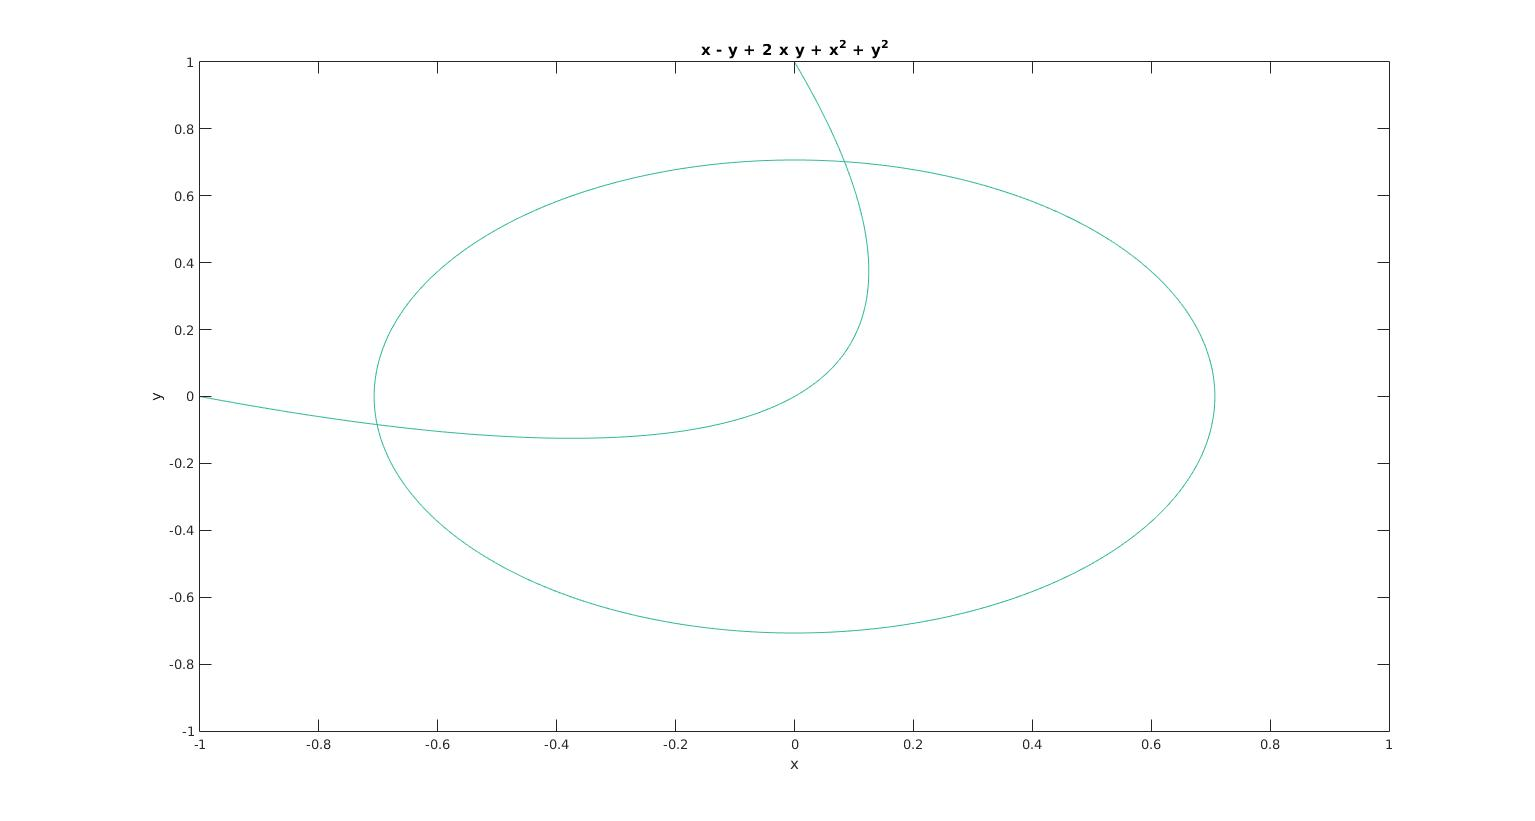
\includegraphics[width=5in]{p8-1.jpg}
\caption{graphing of the two functions}
\end{figure}
\subsection*{8(b)}
To find the roots of the equations, I first construct the resultant by eliminating y. The functions are re-written with x as constants.
\begin{equation*}
\begin{aligned}
p(y) &= 2y^2 + (2x^2-1)\\
q(y) &= y^2 + y(2x-1) + (x^2 +x)
\end{aligned}
\end{equation*}
This then could be use to construct the Q matrix
\begin{equation*}
Q = 
\begin{pmatrix}
2 & 0 & 2x^2-1 & 0\\
0 & 2 & 0 & 2x^2 -1 \\
1 & 2x-1 & x^2+x & 0 \\
0 & 1 & 2x-1 & x^2+x\\ 
\end{pmatrix}
\end{equation*}
Using the symbolic toolkit inside matlab, I could determine the determinant of the matrix, $det(Q) = 16x^4 - 16x^3 + 12x - 1$. Using the build in solver in matlab, I Ire able to solve the 4th degree polynomial, and it gave us 4 different roots (2 real roots and 2 imaginary roots).
\begin{equation*}
\begin{aligned}
   &0.8090 + 0.6360i\\
   &0.8090 - 0.6360i\\
  &-0.7021 \\
   &0.0841 
\end{aligned}
\end{equation*}
Each two real root will give us 2 different y values. To find the correct simultaneous roots for the system, I entered both values into $p(x,y)$ and $q(x,y)$, and picked the roots that are the same for both equations. That gives us the following roots:
\begin{equation*}
\begin{aligned}
	x: -0.7021 \;&y:-0.0840\\
	x: 0.0840 \;&y: 0.7020
\end{aligned}
\end{equation*}
\subsection*{8(c)}
The result of the roots marked on the graph
\begin{figure}[H]
\centering
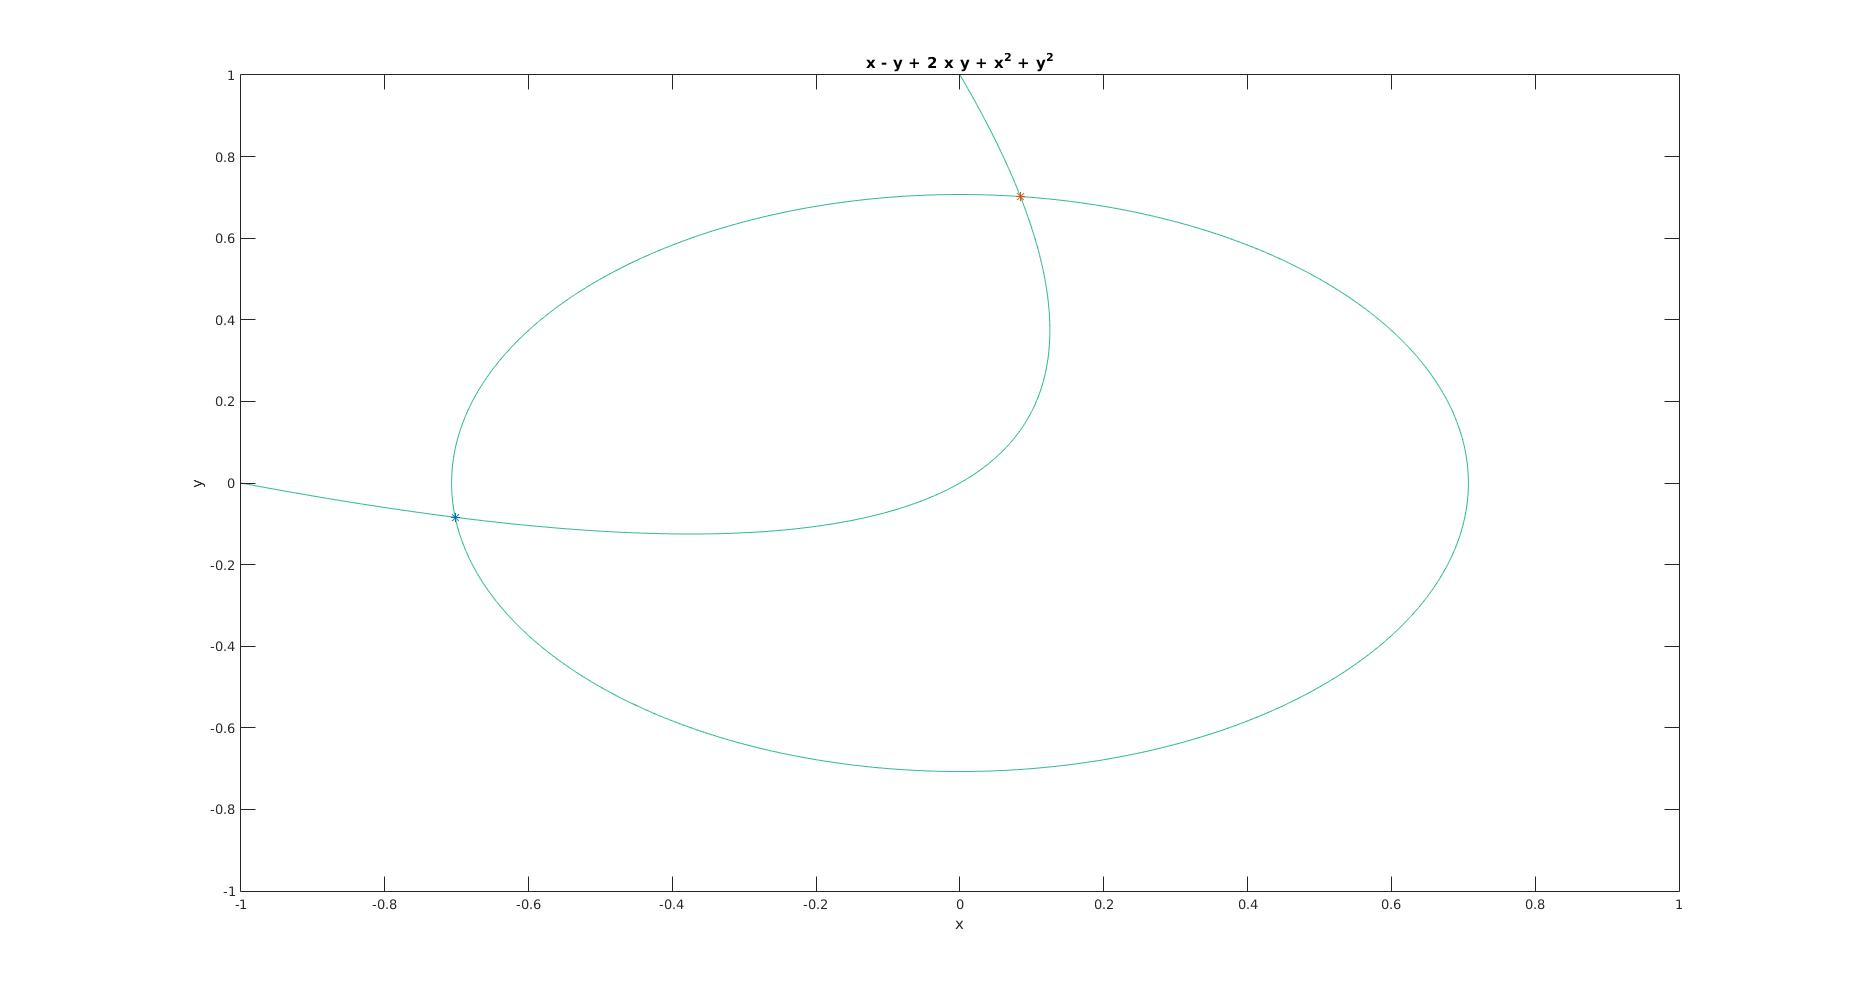
\includegraphics[width=5in]{p8-2-new.jpg}
\caption{graphing of the two functions}
\end{figure}
\section{Q9}
Note: I changed my algorithm as I notice my algorithm was wrong when redoing part 9(c). I explained the new algorithm in part 9(b)
\subsection*{9(b)}
The algorithm is implemented in the function in \textit{interpolatePath.m}.\\
The Algorithm that is used to find the 3 paths are as following:

\begin{algorithm}
\KwResult{Interpolated Path}
Find the path with the closest starting point to the given point\\
That path will be the first path\\
\For{All paths except the first path}{
	\For{All paths except for the first path and the path in the previous loop}{
		continue loop if the signs of $x - y$ for all starting points are not the same\;
		calculate the barycentric values\;
		\If{barycentric values are all $>= 0$ and sum of all values $=1$}{
			\If{area of the triangle created by the three points $<$ minArea}{
				minArea = newArea\;
				save the current path as best path;
			}
		}
	}
}
Interpolated Path = 3 best paths interpolated with barycentric values as their weights\;
\end{algorithm}

To find the barycentric values, I used the linear equation in $9(a)$ and plugged in the values from the three selected points and starting point. Following is the equation used.
\begin{equation*}
\begin{pmatrix}
x^{p_1} & x^{p_2} & x^{p_3} \\
y^{p_1} & y^{p_2} & y^{p_3} \\
1 & 1 & 1 
\end{pmatrix}
\begin{pmatrix}
\alpha_1 \\
\alpha_2 \\
\alpha_3 \\ 
\end{pmatrix}
=
\begin{pmatrix}
startPoint_x \\
startPoint_y \\
1 
\end{pmatrix}
\end{equation*}
The interpolation is a simple linear interpolation with a time factor that interpolate two discrete path steps. The time scale is 0 to 1, where the interval is decided by the user(currently is 0.01). I picked 0 to 1 because how it's commonly use in the computer graphics area as a time scale for drawing curves.
\subsection*{9(c)}
Following is graph with the given starting points. The blue paths are the path use to interpolate the new path(in red)
\begin{figure}[H]
\centering
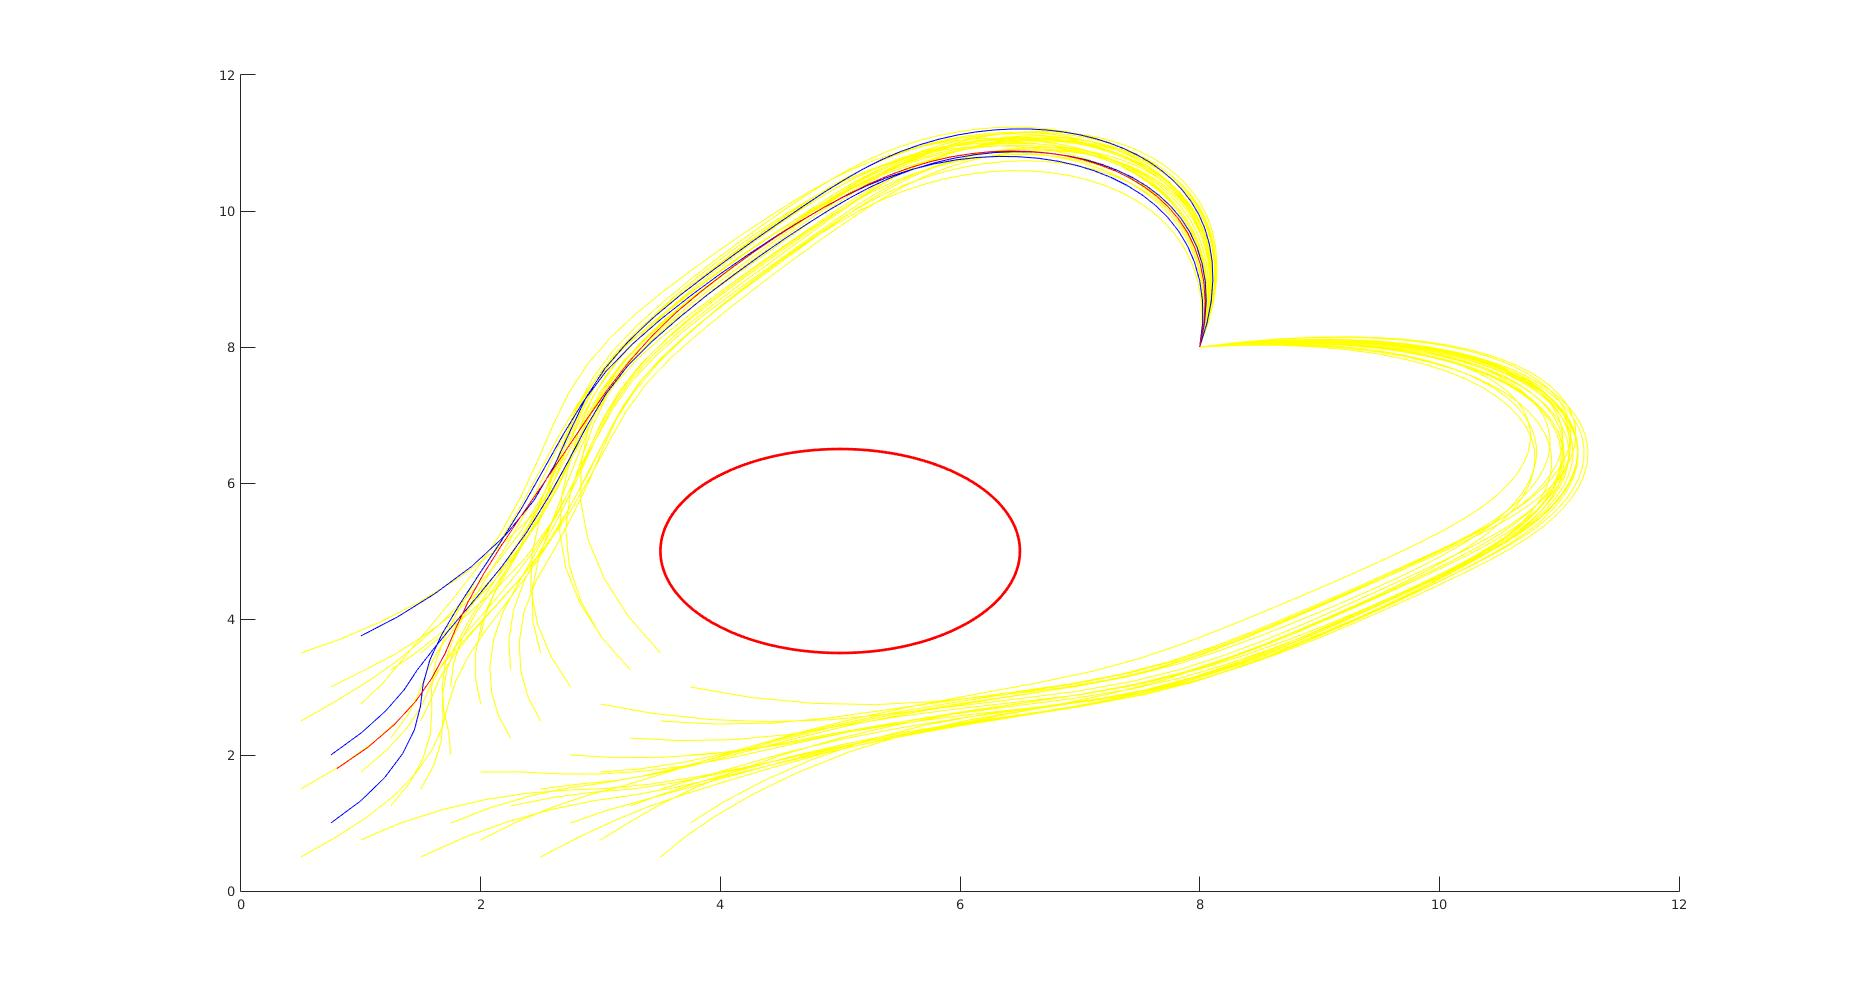
\includegraphics[width=6in]{p9-1.jpg}
\caption{interpolated path with starting point $(0.8, 1.8)$}
\end{figure}
\begin{figure}[H]
\centering
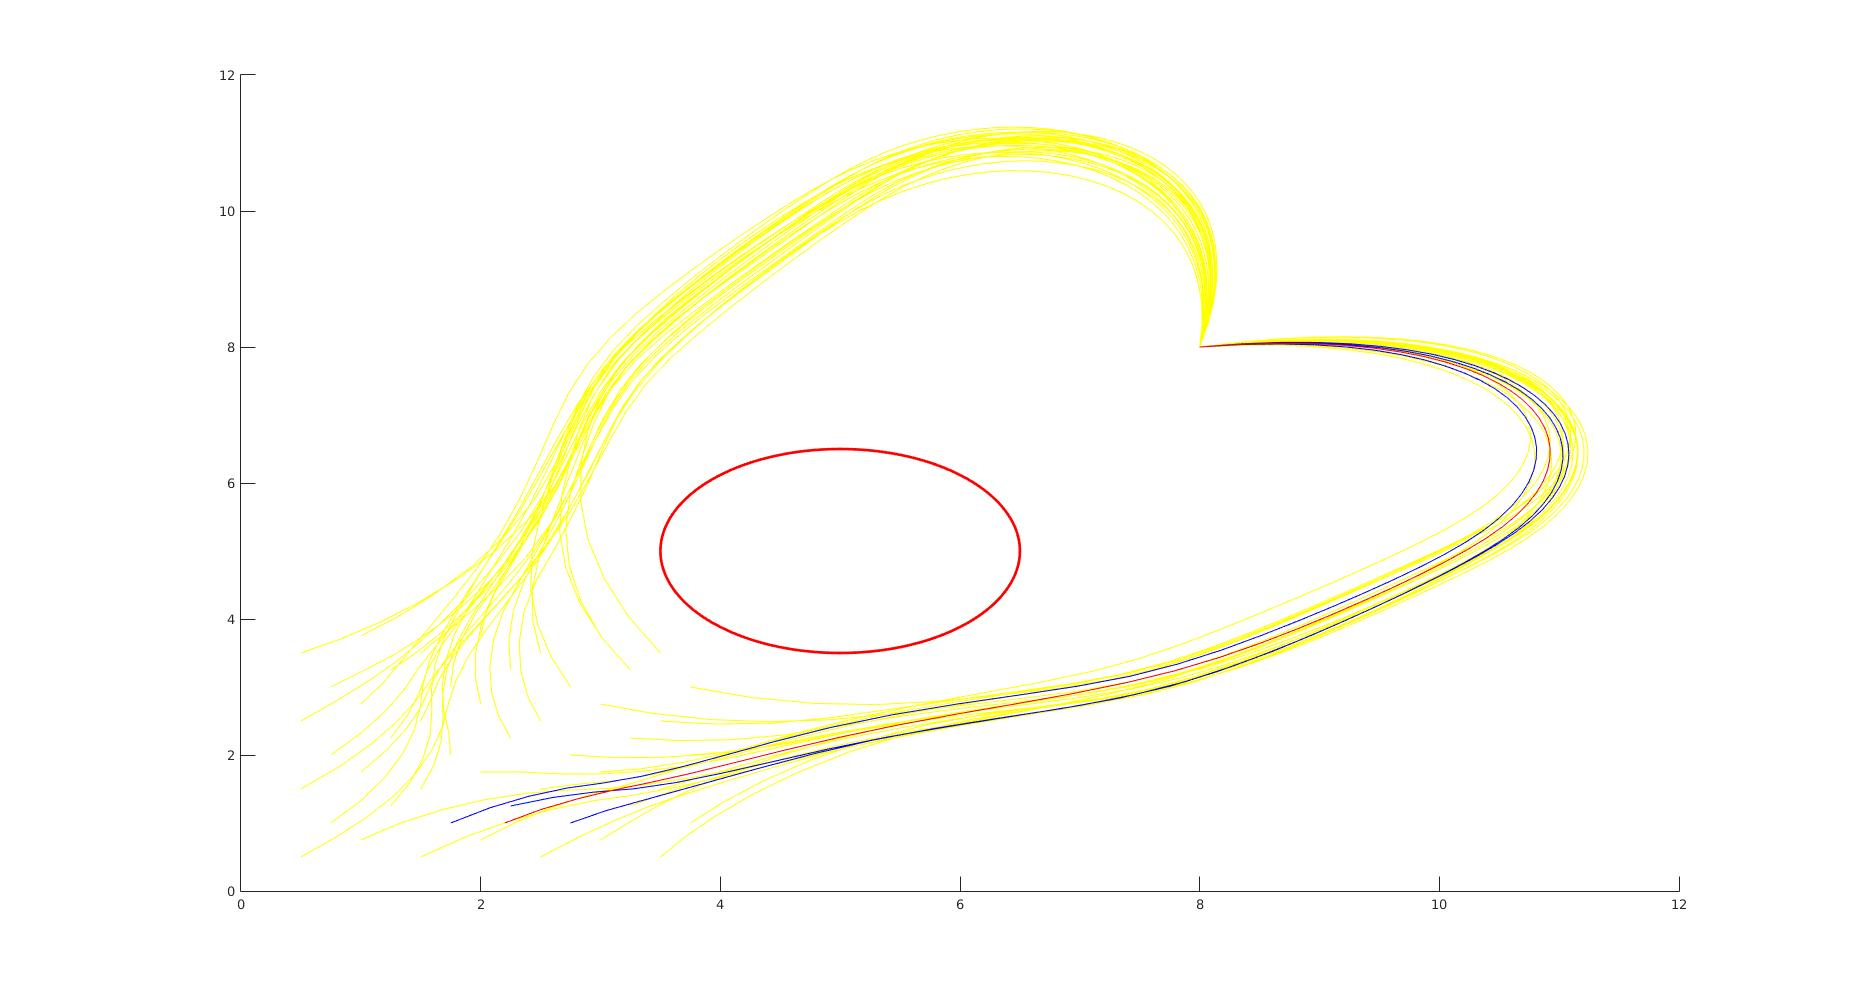
\includegraphics[width=6in]{p9-2.jpg}
\caption{interpolated path with starting point $(2.7, 1.4)$}
\end{figure}
\begin{figure}[H]
\centering
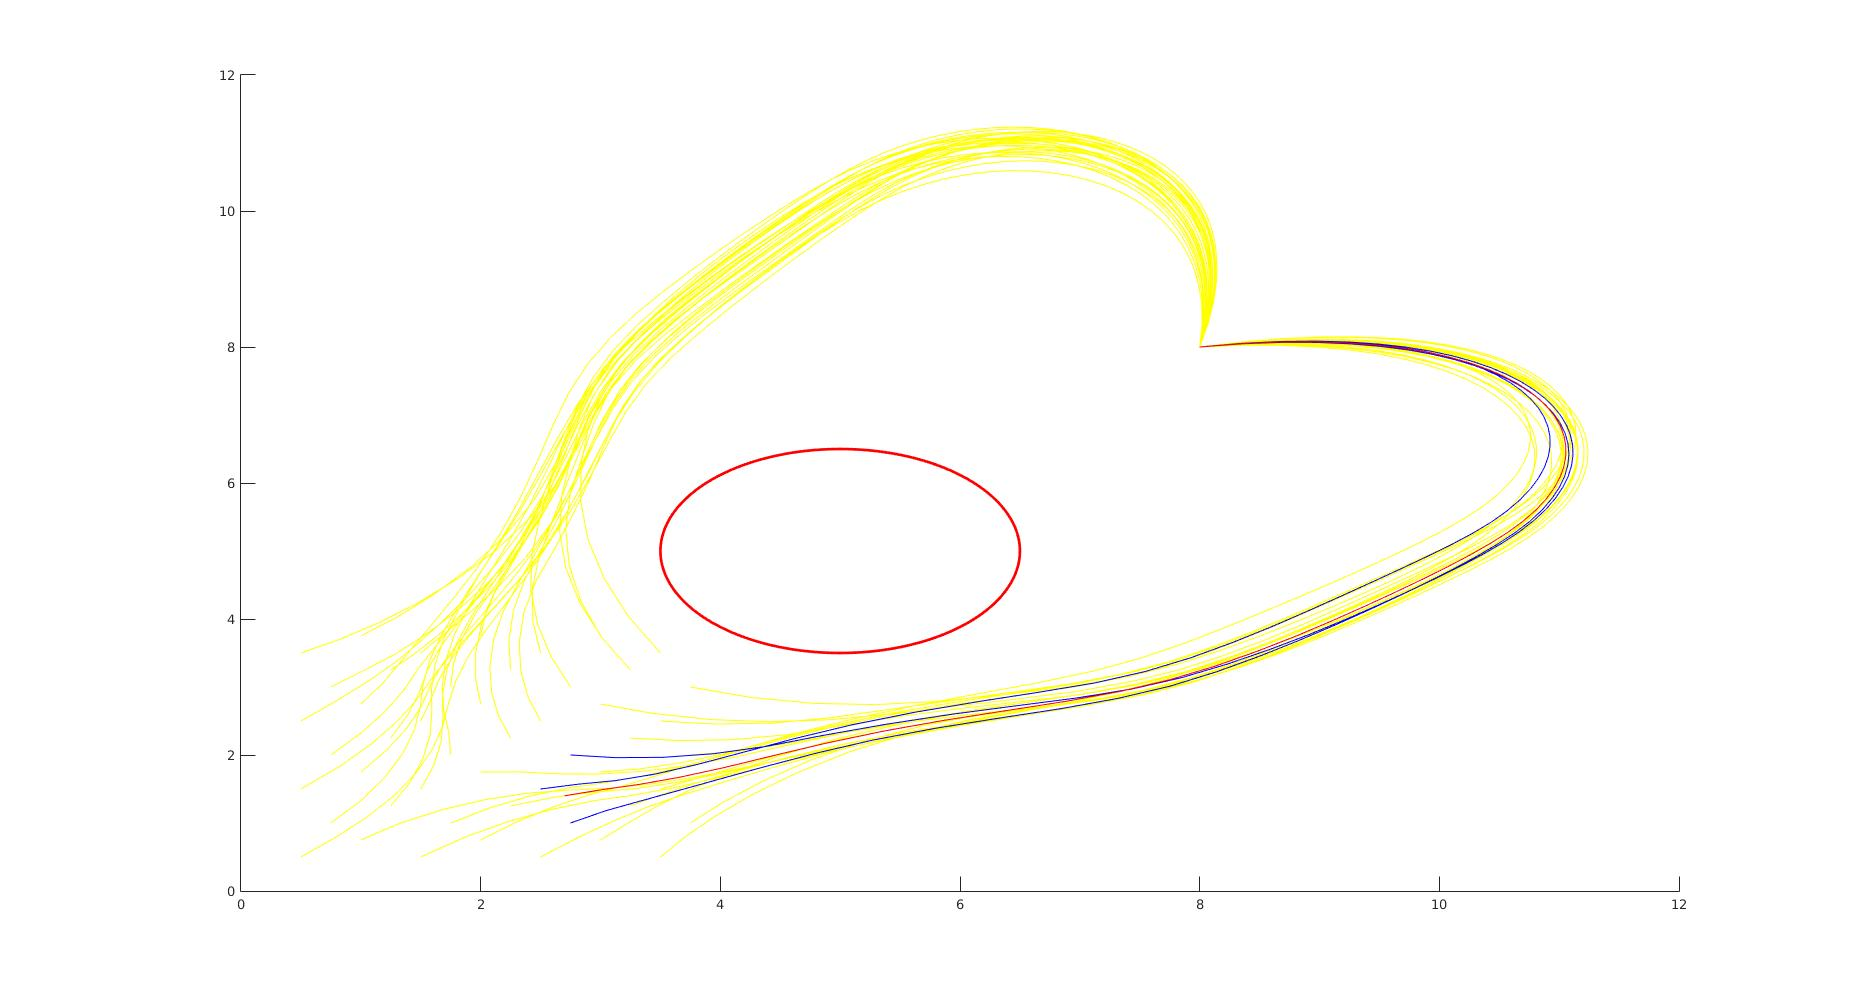
\includegraphics[width=6in]{p9-3.jpg}
\caption{interpolated path with starting point $(2.2, 1.0)$}
\end{figure}

\subsection*{9(d)}
If more obstacles are added into the system, the algorithm needed to modified such that it will select similar path. Currently, the algorithm selects paths from two groups, one where $x - y <= 0$ and $x - y > 0$ based on the first path's membership. This simple equation splits the paths into those following the right and those going from the left. If there are more obstacles, we need to have a method to be able to separate each path into multiple groups where paths in each groups follow a similar trajectory around an obstacle(whether on the right or left). There are multiple ways to achieve this, one would be through visibility group where paths that goes through the same areas will be grouped together. Another possible method is through clustering where a metric(sum of change over the path, average change) is calculated for all path and cluster those with the similar values together and form a new group. Onces we have these groups, we just find the group where the first path is a member(if not, probably find the closest group) pick the 2 other paths from the group that create a triangle with the starting point inside and interpolate the path with those paths. One restriction is that all group must have at least 3 paths to make these methods work.
\end{document}